% !TeX root = ../main.tex

\section{Overview}\label{sec:capability} \label{sec:capacity:overview}

\begin{figure*}[t]
	\centering
	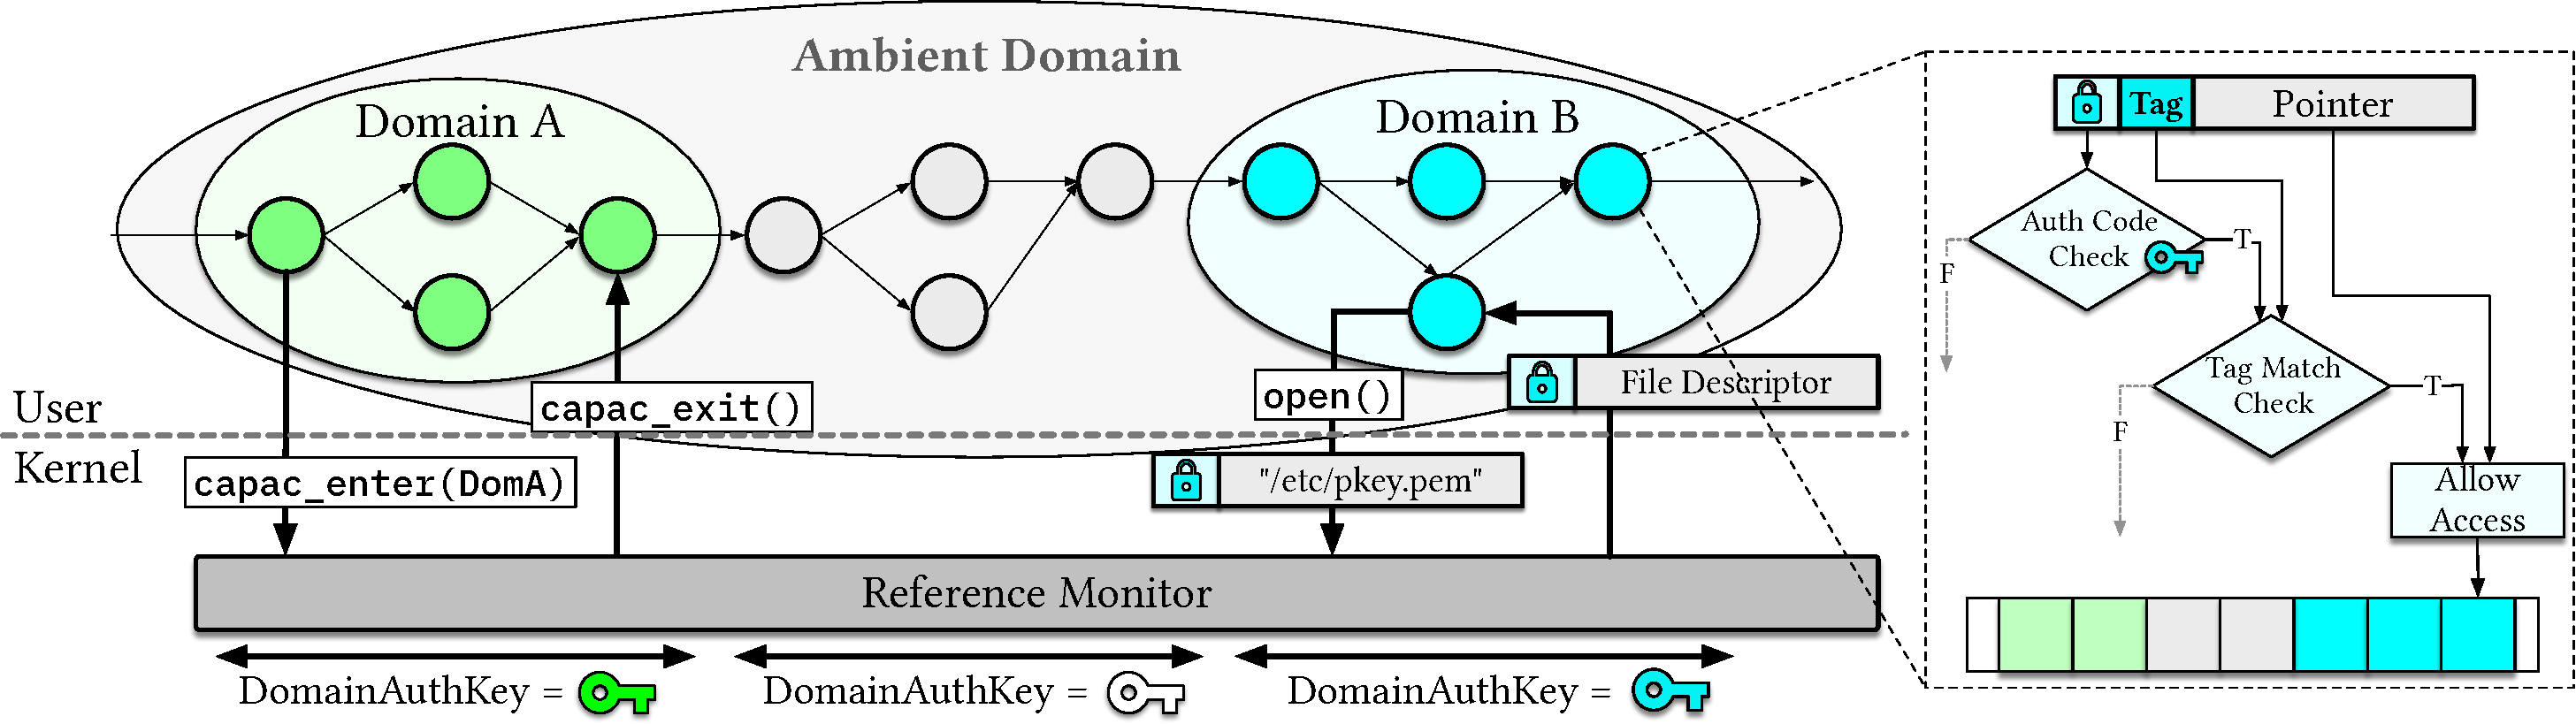
\includegraphics[width=\textwidth]{figures/capacity/capacity-overview-libertine.pdf}
	% 
\includegraphics[width=0.9\textwidth]{images/capacity_overview_new.pdf}
	% \vspace{-1em}
	\caption{Overview of {\thename}'s in-process domains and life-cycle objects protection. }
	\label{fig:capacity:overview}
\end{figure*}

\autoref{fig:capacity:overview} illustrates an overview of \thename.
% \thename establishes intra-process isolation of file and memory objects through capability-based access control principles.
\thename's design demonstrates a comprehensive capability model for file and memory objects access control that can be applied to commodity arm systems that support \gls{pa} and \gls{mte}.
% the design coherently incorporates these hardware security features of the recent and upcoming arm architecture, whose principles and directions exhibit the characteristics of capability. 
\thename's primary objective is to guarantee each domain's exclusive access rights to the sensitive domain-private objects.
it associates each domain, called \emph{a \thename domain}, with a unique \gls{pa} cryptographic key and \emph{switches} the currently activated key using an in-kernel reference monitor before entering a domain.
% \thename then signs the object references with the per-domain keys and authenticates the domain on use, turning them into \emph{unforgable}, \emph{non-reusable} capability tokens.

Consider the common pattern of sensitive object use shown in \autoref{fig:capacity:overview} (Domain B).
First, a file-system \emph{path reference} (\texttt{"/etc/key.pem"}) is used as an argument to the \texttt{open()} \gls{syscall}.
A \emph{file descriptor} to the file object is then obtained.
Finally, the object is loaded into a memory region (e.g., with the \texttt{read()} \gls{syscall}) so the program can interact with it through \emph{pointers} (\texttt{0x00004bfff}...).
In \thename, the creation and usage of three types of resource references are \emph{completely mediated} with a coherent \pamte-based authentication, provided by (1) a lightweight in-kernel reference monitor that efficiently validates path and file descriptor (\fd) references in \gls{syscall} arguments, and (2) \pamte-assisted tagged memory allocation and pointer authentication instrumentation that isolate domain-private memory and their references.

This section provides a high-level overview of \thename's capability model and its programming model. We will delve into the design and implementation of each of \thename's components that enforce its security in \cref{sec:design:impers}, \cref{sec:design:ref-mon}, and \cref{sec:design:instrumentation}.


\subsection{Threat model}
\label{sec:design:threat-model}

We assume that the domains are mutually distrusting.
The program's vulnerabilities can potentially grant adversaries with arbitrary memory manipulation and control-flow subversion primitives, compromising an \thename domain or the \emph{ambient} domain (the rest of the program code not inside \thename domains).
Even so, a compromised domain must not access other domains' private objects.
We assume that the processor and the kernel are trusted and that modern OS security measures, such as the W{$\oplus$}X policy and ASLR, are in place.
Additionally, we deem the program initialization, including the initialization of \thename, free of attacker influence.
We exclude side-channel attacks and microarchitectural attacks from the scope of this paper.

\thename also incorporates the existing backward-edge and forward-edge \gls{cfi} in its implementation and is compatible with recent advances in \gls{pa}-assisted \gls{cfi} techniques.
\gls{pa}-based backward-edge \gls{cfi}~\cite{pac-it-up,qualcomm-pac,pacstack,llvm-ret-addr} authenticates the return addresses on the stack with \key{IB}, which render the traditional attacks (\eg, ROP attacks) that overwrite the return address on the stack infeasible.
\gls{pa}-based forward-edge \gls{cfi}~\cite{kernel-pac,pac-it-up} authenticates code pointers with \key{IA} with its LLVM \emph{ElementType} ID as the modifier, which restricts indirect calls to (1) valid entry points of functions (2) functions of the matching type.


\subsection{Security requirements}
\label{sec:overview:secreq}
The capability principles hold only when the common security requirements for capability are met.
In particular, we observe that \thename must satisfy the following security requirements:

\renewcommand{\labelenumi}{\secreq{R\arabic{enumi}}}
\begin{enumerate}
	\item \emph{Non-impersonatable domains:} \thename must be able to identify and authenticate intra-process domains and prevent impersonation.
	\item \emph{Complete mediation:} all access to file and memory objects must be mediated by \thename.
	\item \emph{Non-reusable references:} \thename domain-private references are only valid within the domain that owns the object.
	\item \emph{Non-forgeable references:} \thename references must not be forged by the adversary.
\end{enumerate}
\renewcommand{\labelenumi}{\arabic{enumi}}

Throughout the rest of this paper, we use the above requirements to analyze and manifest the security guarantees of \thename.
Upholding the security requirements, therefore, is a challenge that must be addressed by \thename's design and implementation.


\subsection{Subjects and Objects}
\label{sec:overview:domains}
% \label{sec:design:domains}
% One of \thename's key differences with previous \gls{ipi} systems~\cite{hakc,erim,hodor} is that it 

% \keypoint{
% 	As shown in \autoref{fig:overview}, \thename's flavor of capability combines domain-based security and object capabilities.
% }
In \thename's capability model, the subjects are subgraphs of program execution that interact with sensitive objects called \emph{\thename domains}.
Program code that does not belong to a domain is called the \emph{ambient} domain.
\thename identifies and authenticates each domain with a unique \gls{pa} key, called the \emph{domain key}.
Each domain is also associated with an \gls{mte} tag for the tagging of the domain's private memory.
We use \key{DB} among the kernel-managed \gls{pa} keys as the domain key.
\key{DA} is the \emph{ambient key} used to sign and authenticate resources accessible by the entire program.
\key{\{IA,IB\}} are reserved for proposed \gls{pa}-based forward-edge and bardward-edge \gls{cfi} defenses~\cite{pac-it-up,pacstack,apple-pac,qualcomm-pac}.

\hdr{Domain switching}
A \thename domain is encapsulated between the APIs \texttt{capac\_enter} and \texttt{capac\_exit}.
% Upon a domain entry, a \thename process  update the activated \gls{mte} tag to that of the destination domain, then informs the in-kernel component to \emph{switch} currently activated domain key.
Domain switching is performed with the help of a lightweight in-kernel reference monitor, as we will describe in \cref{sec:design:switch-auth}.
Upon entering a domain, the userspace program updates its current \gls{mte} tag and requests the reference monitor to switch the currently activating domain authentication key to that of the target domain.
A \emph{per-instance} \gls{pa} modifier is also maintained in both kernel and userspace to identify \emph{instances} of a domain invocation.
\texttt{capac\_exit()} restores the domain key, \gls{mte} tag and modifier to those of the ambient domain.
We do not support the nesting of domains in the current prototype.
% Additionally, \thename can be introduced to flexible isolation boundaries due to its entry gate design, while schemes that employ modifier-based contexts, such as HAKC, require static program and resource partitioning.

\begin{figure}[t]
	\centering
	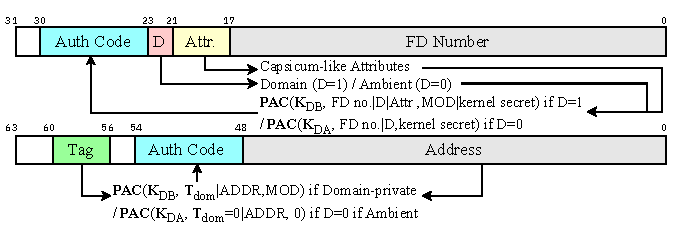
\includegraphics[width=0.95\columnwidth]{figures/capacity/capacity-ref-new.pdf}
	\caption{\thename's reference encapsulation of pointers and file descriptors with cryptographic authentication code (AC).}\label{fig:ref-encapsulation}
\end{figure}

\paragraph{Object encapsulation.}
% \autoref{fig:ref-encapsulation} summarizes how \thename constructs resource references with \gls{pa} and \gls{mte} hardware acceleration.
As summarized by \autoref{fig:ref-encapsulation}, \thename facilities employ \gls{pa} to \emph{sign} private resource references with the domain key and the per-instance modifier (e.g., a unique session ID), engraving the reference ownership into its embedded \gls{ac}.
Before a reference is used to access some resource, \thename \emph{authenticates} its \gls{ac} with the currently activating domain key and modifier before granting the access.
Consequently, object references are turned into non-forgeable (\srforge) \emph{capability tokens} that are valid only when the context is within their owner domain.
By simply switching the authentication key, \thename prevents cross-domain reusing of both kernel and userspace object references (\srreuse).
% while also avoiding the need for complex modifier management.

We introduce the \emph{ambient objects}, non-private and accessible from all domains, \eg, global variables and non-sensitive files, to avoid the programming model becoming too restrictive.
All references to ambient objects are to be signed and authenticated with \key{DA}.
The ambient memory objects are given a \tagnum{Dom} of $0$, which makes all untagged memory pointers ambient memory references, and only the deliberately tagged pointers become references to domain-private memory.
To facilitate multi-domain interactions, \thename also supports the \emph{delegation} of references.
When a reference delegation request is received, \thename first authenticates the reference to prevent delegation of non-owned resources (\srimper), then \emph{re-signed} it with the target's domain key and instance modifier.
Especially for memory reference delegation, \thename compares the pointee memory's tag with the pointer's tag before recoloring both to the target domain's memory.

\begin{listing}[t]
	\centering
\begin{minipage}[b][11cm][b]{.95\textwidth}
\begin{minted}[escapeinside=||]{c}
  capac_init(...);
  ...
  // |{\tt \key{DB} $=$ \key{Dom_{crypt}}, Dom$_{curr}$ $=$ Dom$_{crypt}$, $\texttt{Mod}_{curr}$ $=$ ctx->id }|
  capac_enter(DOM_CRYPTO, ctx->id);
  load_secret(|\hlblue{ctx}|, |\hlblue{\textquotesingle{}\textquotesingle{}secret.key\textquotesingle{}\textquotesingle{}}|);
  encrypt(|\hlblue{ctx}|, |\hlgray{req}|);
  capac_exit();
  ...
void load_secret(|{\textcolor{blue}{\underline{\tt{}DOM\_PRIV}}}| crypto_ctx_t* |\hlblue{ctx}|,
                     const char * |\hlblue{key\_path}|){
  // Import the secret key from the filesystem
  int |\hlblue{fd}|  |\hfill\action{FD-Sign}|
      = open(|\hlblue{key\_path}|, O_RDONLY); |\hfill\action{PATH-Auth}|
  |\hlblue{ctx->secret\_key}| = capac_malloc(KEY_LEN + 1); |\hfill\action{PTR-Sign}|
  read(|\hlblue{fd}|, |\hlblue{ctx->secret\_key}|, KEY_LEN); |\hfill\action{FD-Auth}/\action{PTR-Auth}|
  ...
}
|\textcolor{blue}{\underline{\tt{}DOM\_PRIV\_FUNC}}|  // Isolate function stack frame
void encrypt(|\textcolor{blue}{\underline{\tt{}DOM\_PRIV}}| crypto_ctx_t* |\hlblue{ctx}|, req_t* |\hlgray{req}|) {
  // Use the secret key to encrypt a plaintext string
  for (int i = 0; i < KEY_LEN; i++)
      |\hlgray{req->ciphertext}|[i] |\hfill\actionambient{PTR-Auth}|
          = |\hlblue{ctx->secret\_key}|[i]|\hfill\action{PTR-Auth}|
            ^ |\hlgray{req->plaintext}|[i];  |\hfill\actionambient{PTR-Auth}|
}
\end{minted}
% \vspace{-5em}
\end{minipage}
\begin{minipage}{.95\textwidth}
\begin{flushleft}
{\noindent\hlblue{\ \ \ \ \ \ \ \ } : Domain-private references
\hspace{0.5em} \hlgray{\ \ \ \ \ \ \ \ } : Ambient references
\\
\action{Action} : \thename actions
\hspace{0.5em} \textcolor{blue}{\underline{\tt{}ANNOT}}: \thename annotations
}
\end{flushleft}
\end{minipage}

	\caption{Example of \thename's programming model, annotated with \thename references and their enforcement.}
	\label{fig:code-example}
\end{listing}

\begin{table*}[t]
	\small
	\centering
	\begin{tabularx}{.98\textwidth}{lXX}
		\toprule
		                                                                       & \thead{API \& Compiler Annotation}                              & \thead{Description}                                                                        \\
		\midrule
		\multirow{6}{*}[-0.5em]{\thead{\begin{sideways}API\end{sideways}}}     & \texttt{capac\_init(configurations)}                            & Initializes \thename facilities, assigns \cpath to domains, enables syscall authentication \\
		\cline{2-3}
		                                                                       & \texttt{capac\_enter(target\_id, mod)}/\texttt{capac\_exit()}   & Enters the target domain/Exits to the ambient domain                                       \\

		\cline{2-3}
		                                                                       & \texttt{capac\_limit\_fd(fd, cap\_mask)}                        & Limit the capabilities of an \fd                                                           \\

		\cline{2-3}
		                                                                       & \texttt{capac\_delegate\_fd(fd, target\_id, mod, cap\_mask)}    & Limits the capabilities and delegate an \fd to the target domain                           \\

		\cline{2-3}
		                                                                       & \texttt{capac\_malloc(size)}/\texttt{capac\_free(ptr)}          & Allocates/frees memory tagged with the currently active domain                             \\

		\cline{2-3}
		                                                                       & \texttt{capac\_delegate\_ptr(ptr\_loc, size, target\_dom, mod)} & Delegates an in-memory pointer to \texttt{target\_dom} and also re-colors the memory       \\
		\midrule
		\multirow{1}{*}[0em]{\thead{\begin{sideways}Annotation\end{sideways}}} & \texttt{DOM\_PRIV\_FUNC}                                        & Tags function’s stack frame with the currently executing domain’s tag (\tagnum{Dom})       \\

		\cline{2-3}
		                                                                       & \texttt{DOM\_PRIV}                                              & Marks a \emph{source} domain-private pointer for taint analysis.                           \\
		% & \texttt{AMBIENT}                                               & Marks a \emph{source} ambient pointer. Taint analysis will untaint derived pointers.                       \\
		\bottomrule
	\end{tabularx}
	\caption{\thename APIs and program annotations}\label{tab:apis}
\end{table*}




\subsection{Programming model overview}
% \section{Design and Implementation}
\label{sec:enforcement}
\label{sec:implementation}

\label{sec:design:prog-model}


\keypoint{
	A programmer interacts with \thename through a set of well-defined APIs provided by the runtime library and program \emph{annotations} that direct the program instrumentation, shown in \autoref{tab:apis}.
}
We demonstrate the programmer's perspective when retrofits intra-process capabilities into programs through a quintessential example of secret import and uses in \autoref{fig:code-example}.
% In the example, the program loads a file that contains the secret key into memory and uses it to perform encryption.



The programmer first conceptually defines in-program domains (\eg, \texttt{DOM\_CRYPTO}) within the program with respect to the domain-private resources.
The subprogram interval is enclosed by \texttt{capac\_enter()} and \texttt{capac\_exit()} (lines $4$ and  $7$), and each interval is paired with a domain key.
% The domain entry additionally takes an instance-specific modifier as the second argument.
In the example, \texttt{ctx->id} contains the unique ID for the encryption context, which is set as the currently activated \gls{pa} modifier for \texttt{DOM\_CRYPTO}.
A domain can span a few function calls, as shown in the example.
The domain entrance cannot be nested; however, \thename is designed to support the sharing of functions between domains.


The programmer then identifies domain-private objects and their references.
In the case of file(-like) objects, a list of domain-to-file mappings is provided as an argument to \texttt{capac\_init()} (line $1$) to notify the reference monitor of the domain ownership of file resources.
Afterward, the reference monitor automatically authenticates any path and \fd references in the \gls{syscall} arguments (lines $11$, $12$, $14$) and issues \fds signed with their owner domain when \fds are created.
For memory objects, the programmer must mark the domain-private region containing the object and its domain-private pointer references.
To allocate domain-private memory, the programmer either changes their allocation site to use \texttt{capac\_malloc} (line $13$), which allocates memory tagged with the domain's tag and returns a tagged pointer, or uses \texttt{DOM\_PRIV\_FUNC} (line $17$) to direct the instrumentation to isolate the function's stack frame.
On \texttt{DOM\_PRIV\_FUNC}-annotated functions, the function is instrumented such that the stack frame is \emph{tagged} with the currently executing domain's tag number and reverted upon function return.
Then, the programmer applies \texttt{DOM\_PRIV} (line $18$) to the \emph{source} domain-private pointer.
From then on, the pointer is \emph{taint-tracked} to mark all derived references to the object within the function.
\thename then instruments \gls{pa}-based signing/authentication with the domain key of tracked pointers, including the member variables (\eg, \texttt{ctx->secret\_key}) (lines 13, 14, 21).


